\documentclass[11pt]{article}
\usepackage{fullpage,amsmath,mathtools, algorithm2e, forest}
\usepackage{graphicx}
\graphicspath{ {./images/} }
\title{COMP4107 - Assignment 1}
\author{Student Name: Yunkai Wang\\
\text{Student Number: 100968473}\\\\
Student Name: Jules Kuehn\\
\text{Student Number: 100661464}}
\date{Fall 2018}
\begin{document}
\maketitle
\begin{enumerate}

\item Question 1

\item Question 2\newline
Implementation for question 2 can be found in q2.py. The results is\\
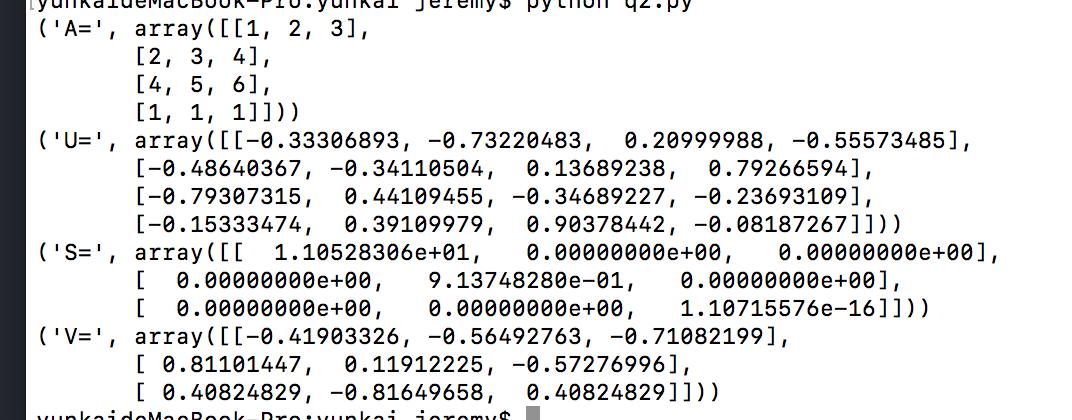
\includegraphics{q2_result}

\item Question 3\newline
Implementation for question 3 can be found in q3.py. The rank-2 approximation and $||A-A_2||$ is\\
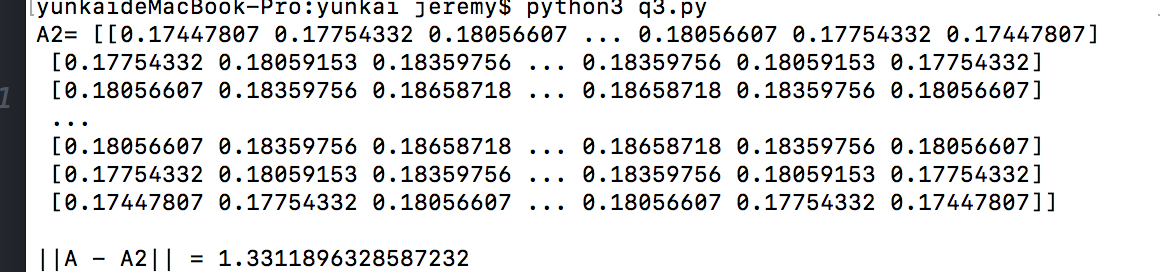
\includegraphics{q3_result}

\item Question 4\newline
Implementation for question 4 can be found in q4.py. The only learning rate that will work is when $ε = 0.01$, which will lead to the correct result with $\approx 420$ iterations. The other ones won't work as we are descending too quickly, and therefore we will miss the correct answer and failed to come back. We set the program to stop

\item Question 5\newline

\item Question 6\newline

\item Question 7\newline

\end{enumerate}
\end{document}